
\chapter{Kravspecifikation}
\section{Use case diagram}
\begin{figure}[H]
	\centering
	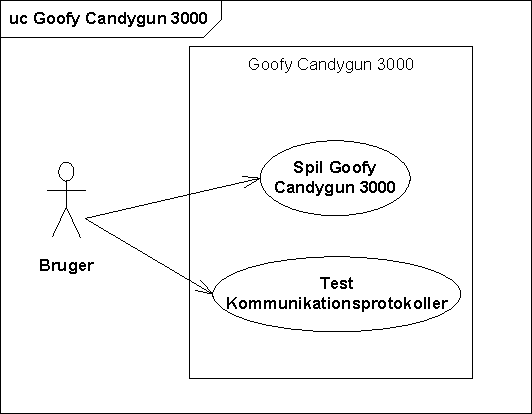
\includegraphics[]{Kravspecifikation/images/usecaseDiagram}
	\caption{Use case diagram for produktet}
	\label{ref:usecaseDiagram}
\end{figure}


\section{Aktør kontekst diagram}
\begin{figure}[H]
	\centering
	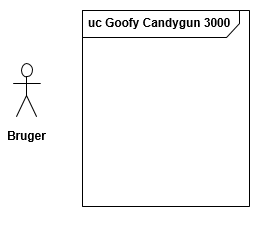
\includegraphics[]{Kravspecifikation/images/kontekstDiagram}
	\caption{Kontekst diagram for produktet}
	\label{ref:kontekstDiagram}
\end{figure}

\section{Aktør beskrivelse}
I 'Goofy CandyGun 3000' systemet er der kun 1 primær aktør, nemlig brugeren. Det er brugeren der initierer systemet, ved at vælge spiltype på brugerinterfacet, og brugeren har også mulighed for at stoppe spillet igen fra samme brugerinterface. Brugeren vil under spillet interagere med systemet vha. Wii-Nunchucken. 


\section{Fully dressed use case}
\begin{tabular}{|>{\hspace{0pt}}p{3cm}  |>{\hspace{0pt}}p{9cm}|}
	\hline
	\textbf{Navn} & Spil Goofy Candygun 3000\\ \hline
	\textbf{Mål} & At spille spillet\\ \hline
	\textbf{Initiering} & Bruger\\ \hline
	\textbf{Aktører} & Bruger\\ \hline
	\textbf{Antal samtidige forekomster} & Ingen \\ \hline
	\textbf{Prækondition} & Spillet og kanonen er operationel \\ \hline
	\textbf{Postkondition} &  Brugeren har færdiggjort spillet \\ \hline
	\textbf{Hovedscenarie} & \begin{enumerate}
		\item Bruger vælger spiltype på brugergrænsefladen
		\subitem [Extension 1: Brugeren vælger 2 player mode] 
		\item Brugeren vælger antal skud til runden
		\item Brugeren fylder magasin med slik tilsvarende antal skud
		\item Brugeren indstiller kanon med analog stick på Wii-nunchuck
		\item Bruger udløser kanonen med Wii-nunchucks trigger
		\item Systemet lader et nyt skud
		\item Brugergrænsefladen opdateres med spillets statistikker
		\item Punkt 4 til 6 gentages indtil skuddene er opbrugt 
		\subitem[Extension 2: Bruger afslutter det igangværende spil]
		\item Brugergrænseflade viser afslutningsinfo for runden
		\item Brugeren afslutter runden
		\item Brugergrænsefladen vender tilbage til starttilstanden
	\end{enumerate}\\ \hline
	\textbf{Udvidelser/ undtagelser} & \textbf{[Extension 1: Brugeren vælger 2 player mode]} \newline \begin{enumerate} 
		\item Punkt 4 til 7 i hovedscenariet gennemføres
		\item Brugeren overdrager Wii-nunchuck til den anden bruger
		\item Punkt 1 til 2 gentages indtil skuddene er opbrugt
		\item Use casen genoptages fra punkt 8
		\end{enumerate}
		\textbf{[Extension 2: Bruger afslutter det igangværende spil]} \newline \begin{enumerate}
		\item Brugergrænsefladen vender tilbage til starttilstanden
		\item Use casen afsluttes
		\end{enumerate}\\ \hline
\end{tabular}

\section{Ikke funktionelle krav}
\begin{itemize}
	\item Kanonen drejes 0-70 grader vertikalt (+- 5 grader)
	\item Kanonen kan drejes +-45 grader horizontalt
	\item Kanonen kan afyre slik af typen M\&M's, Skittles eller Pinnochio kugler (Eller andre kugler af X mm i diameter +- Y mm)
	
	\item Brugerfladen er en grafiskbrugergrænseflade (Ikke terminalbaseret)
	\item Kanonen skal kunne afyre sit projektil minimum 1 meter.
	\item Kanonen må max være 40cm høj, bred og 'dyb'
	
	\item 
\end{itemize}